\pagestyle{empty}
\cleardoublepage
\pagestyle{fancy}

\chapter{Algoritmo Proposto}\label{cap3}

\section{Introdução}\label{cap3:intro}

Esta seção demonstra detalhes de implementação do algoritmo proposto para o balanceamento de carga dinâmico em aglomerados de GPUs.


\section{Algoritmo}
Visão geral. O algoritmo proposto determina o tamanho do bloco ideal por processador usando uma abordagem de rebalanceamentos. Inicialmente, são encontradas as velocidades relativas de cada processador. Com esses valores são feitas curvas com um certo número de pontos e a partir dessas curvas geram-se modelos de execução de cada processador. O intuito é realizar uma regreessão sobre esses pontos e gerar uma curva que nos permite determinar o comportamento do modelo para cada processador. Processa-se uma quantidade relativamente pequena de dados, cujo limite superior é definido como uma percentagem fixa do total de dados, para a obtenção desses pontos. Começa-se com os maiores blocos possíveis para otimizar o tempo de execução, reduzindo o tamanho dos blocos com o passar dos rebalanceamentos. O tamanho do bloco diminui progressivamente à medida que a computação trabalha no sentido final para que todas as unidades de execução completem quase ao mesmo tempo. O algoritmo se resume a duas fases: uma fase chamada fase de adaptação e outra fase chamada fase de conclusão. O objetivo da primeira fase é determinar um peso a cada processador, que é utilizado na fase de conclusão do algoritmo.

Os pesos são calculados com base no tempo total necessário para a transferência de dados e o tempo de execução. Isto é essencial para o balancemanto de carga preciso.

Fase de adaptação: Esta fase encontra a velocidade relativa das unidades de computação que resultam em pesos para serem usado na fase de conclusão. O principal desafio é a de manter a fase inicial de adaptação o mais curta possível de modo a que a maior parte dos dados seja deixada para a fase de conclusão. 

Para conseguir isso, começa-se com tamanhos de blocos pequenos inicialmente e aumentá-os gradualmente com base no desempenho observado até que seja possivel determinar o cálculo preciso para os pesos para cada dispositivo.

A fase de adaptação primeiro mede o número de iterações concluídas na etapa anterior por unidade de tempo. Isto fornece o peso computacional, uma velocidade relativa de processamento para o último passo . Se a mudança de pesos entre o passo anterior e etapa atual é inferior a MIN altera-se a taxa ( que é definido como 0,01, o qual é considerado estável). Caso contrário, é preciso aumentar o tamanho do bloco para a próxima etapa.

A fim de alcançar a convergência dos pesos, estima-se uma curva para cada processador usando o método de Gauss-Newton. Uma vez que os parâmetros são obtidos, estima-se um peso computacional estável para cada processador e assim um tamanho estimado do bloco para cada processador.

Depois que o tamanho estimado do bloco é enviado para o processador, na solicitação de bloco seguinte, o algoritmo verifica se a estimativa é precisa, calculando o peso computacional novamente. Se a mudança de peso ainda não é estável, o processo de estimativa continua.

Uma vez que um peso computacional é  estável, o algoritmo continua aumentando tamanhos de bloco para outros processadores instáveis ​​até que todos os pesos se tornem estáveis ou uma percentagem fixa (20\%) de todos os dados serem processados. O último caso é um limite superior forçado para limitar a duração da fase de adaptação .

Fase de conclusão. Uma vez que todos os pesos são estáveis​​, o algoritmo passa para a fase de conclusão. Tamanhos de blocos da fase de adaptação não são mais usados. Em vez disso, o algoritmo usa o Guided Self-Scheduling modificado (MGSS) para encontrar o tamanho dos blocos corretos. A fase de conclusão integra pesos computacionais calculados na etapa anterior em MGSS. Eq. \ref{eq: gss} é a fórmula original GSS, que simplesmente divide o restante número de iterações de R para o número total de processadores P. MGSS utiliza Eq. \ref{eq: mgss} que distribui a R processadores proporcional ao seu peso $w_i$ calculado.

\begin{equation}
 	B = R/P
\end{equation}

\begin{equation}
 	B = R w_i/ \sum_{j=1}ˆ{P} w_j
\end{equation}

MGSS é mais adequado com a computação heterogênea porque ele começa com o maior tamanho de bloco possível e aceleradores são melhor utilizados com tamanhos de blocos maiores. Com os pesos computacionais estimado com precisão, a prova para o GSS original é válida para o MGSS. Isto é devido ao fato de os tamanhos de bloco diferentes calculados para diferentes processadores para o mesmo número de iterações restante terá sempre a mesma quantidade de tempo, porque pesos computacionais causam distribuição proporcional de blocos. 

\section{Implementação}
A implementação foi feita no arcabouço StarPU na linguagem C. Para cada dispositivo foi programado um codelet, com as caractereisticas dos dispositivos. A codelet é uma estrutura que representa uma função computaciona;. Cada codelet pode conter uma implementação do mesmo kernel em diferente arquiteturas (exemplo, CUDA, x86). 

\section{Resultados}

\subsection{Multiplicação de Matrizes}

A figura \ref{fig:1maquina} apresenta o algoritmo executando em uma única máquina. Neste caso o problema tratado é o de multiplicação de matrizes, com complexidade  $O(nˆ2)$. Nota-se que no caso do algoritmo proposto chamado de dinâmico e o HDSS, praticamente não há diferenças significativas na execução.

\begin{figure}[htb]
	\begin{center}
	\centering
			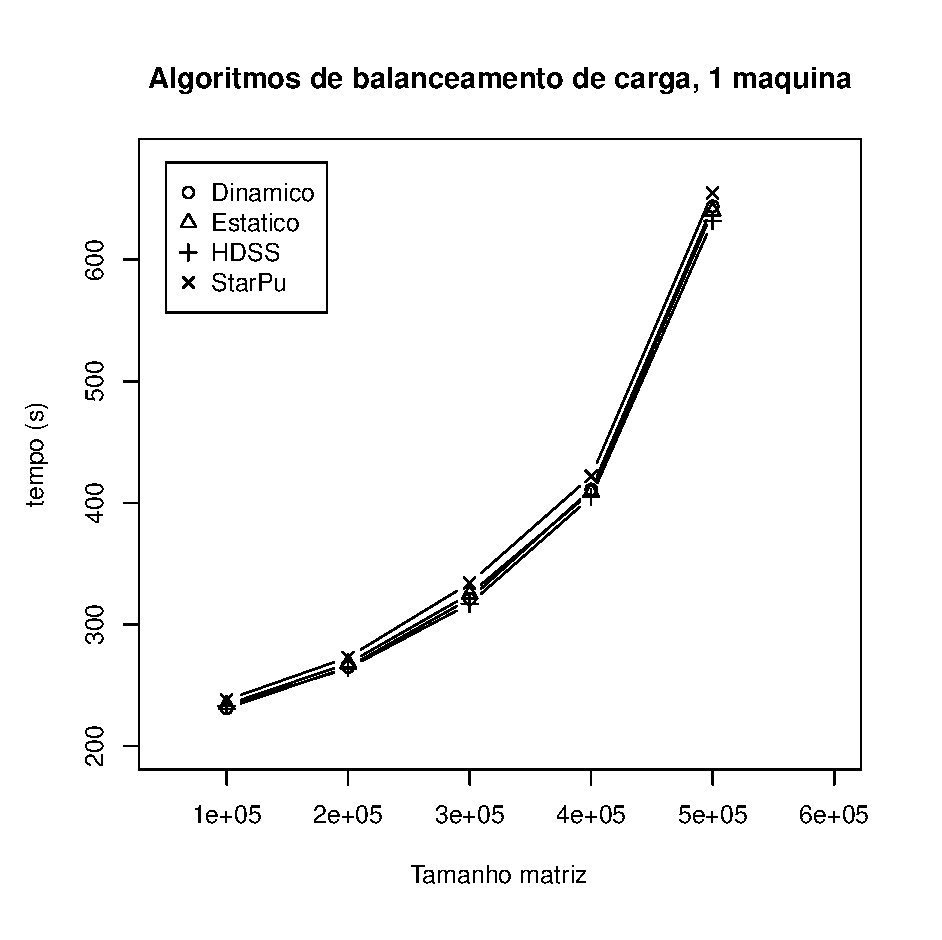
\includegraphics[scale=0.6]{1maquina.eps}
	\caption{Execução do algoritmo em uma máquina}
	\label{fig:1maquina}
	\end{center}
\end{figure}

A figura \ref{fig:2maquina} apresenta o algoritmo executando em duas máquinas.  Neste caso o algoritmo dinâmico leva uma leve vantagem em relação ao HDSS, mas ainda não siginificativa.

\begin{figure}[htb]
	\begin{center}
	\centering
			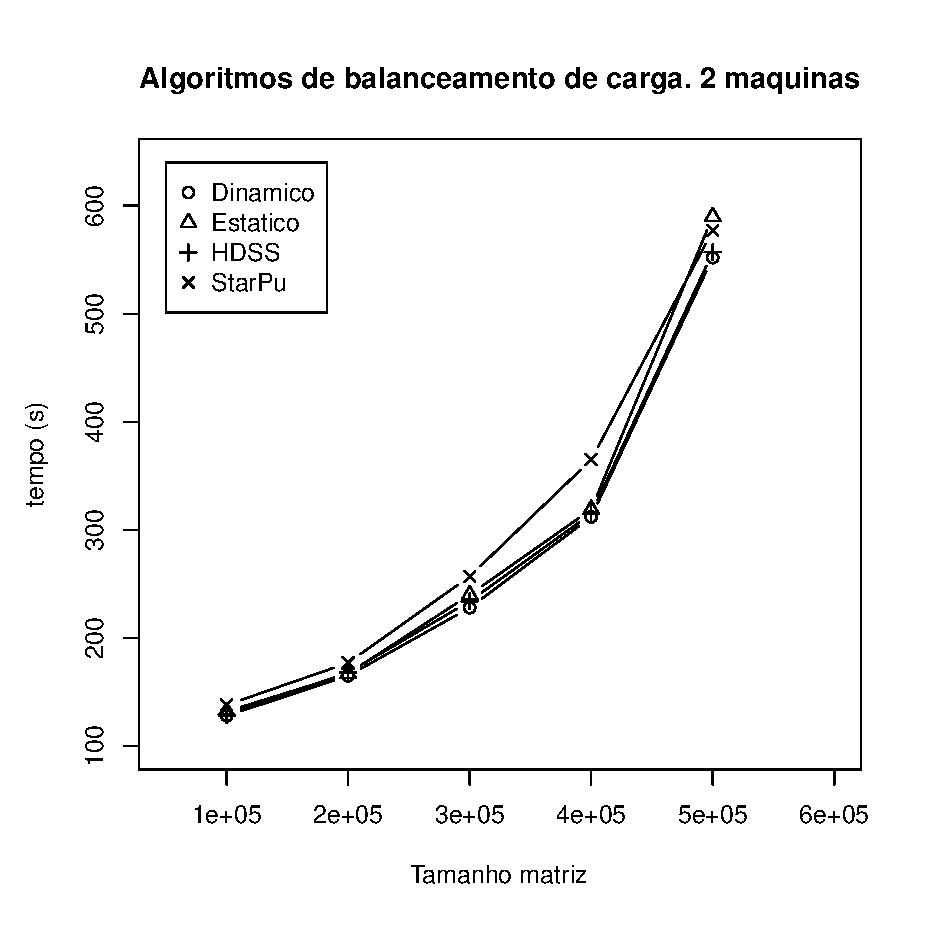
\includegraphics[scale=0.6]{2maquinas.eps}
	\caption{Execução do algoritmo em duas máquinas)}
	\label{fig:2maquina}
	\end{center}
\end{figure}


A figura \ref{fig:3maquina} apresenta o algoritmo executando em três máquinas.  No último caso, oo dinâmico apresentou uma vantagem maior em relação ao HDSS, o que nos revela uma vantagem mais relevante em meios mais hetererogêneos. 

\begin{figure}[htb]
	\begin{center}
	\centering
			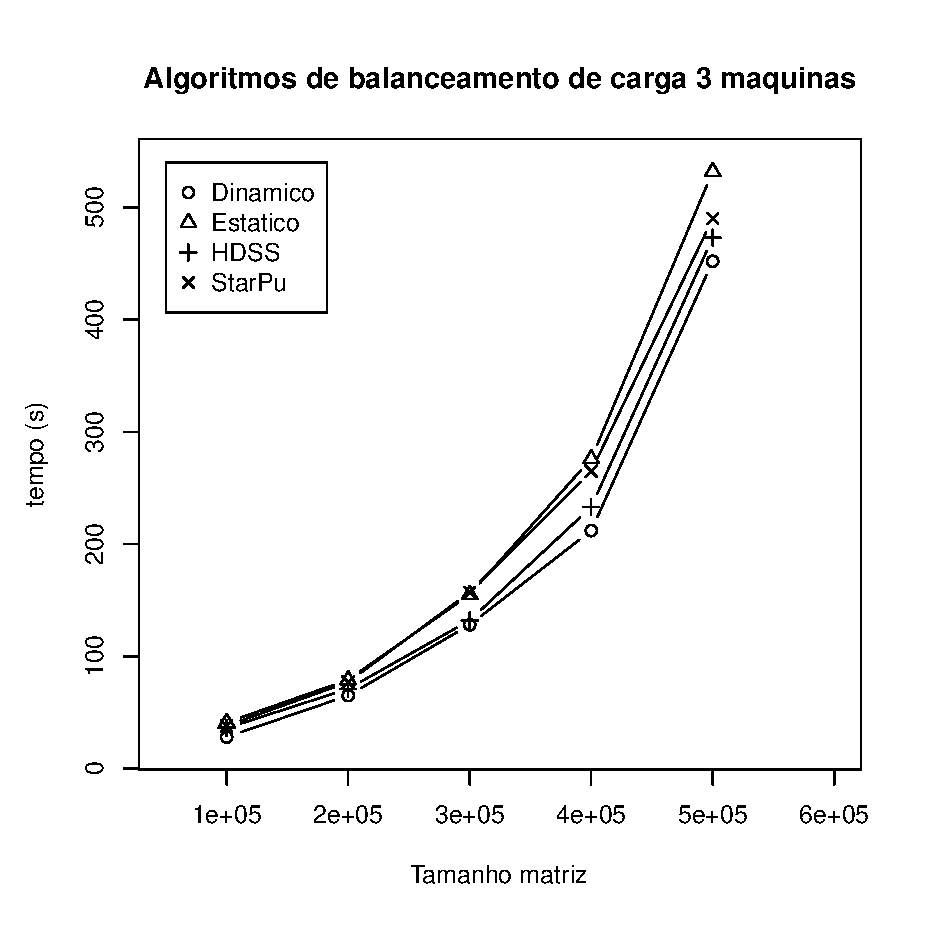
\includegraphics[scale=0.6]{3maquinas.eps}
	\caption{Execução do algoritmo em três máquinas)}
	\label{fig:3maquina}
	\end{center}
\end{figure}

A razão da maior adaptabilidade do algorimto perante os outros algortimos é devido ao método de Newton utilizado nos rebalanceamentos, no faz com que em meios heterogêneos a resolução do sistema de equações seja feita de forma mais eficiente, em relação por exemplo o HDSS, que realiza uma distribuição uniforme da carga na fase de conclusão.



\begin{figure}[htb]
	\begin{center}
	\centering
			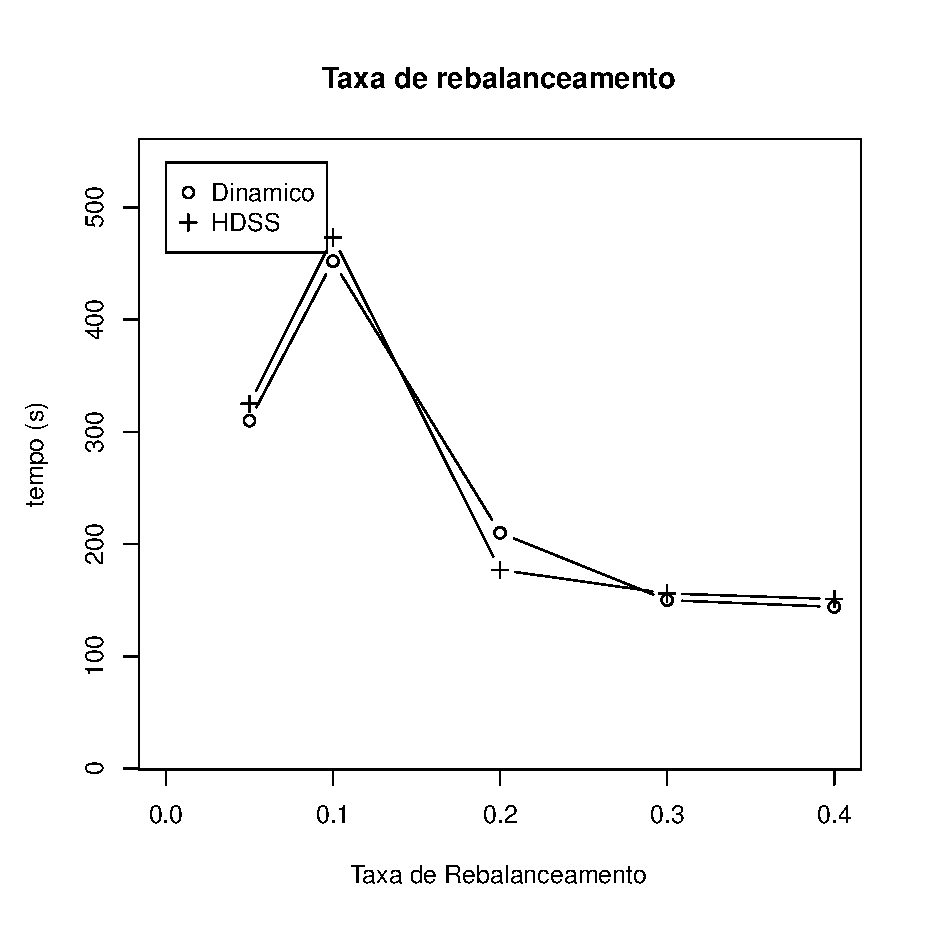
\includegraphics[scale=0.6]{TaxaRebalancemento.eps}
	\caption{Execução do algoritmo em três máquinas, alterando a taxa de rebalancemanto)}
	\label{fig:rebalanceamento}
	\end{center}
\end{figure}

Na figura \ref{fig:rebalanceamento} é variada a taxa de rebalancemento, o que influiencia a quantidade de vezes que é feito o rebalanceamento. Se a quantidade de rebalancemento for elevada o algoritmo faz varios rebalancemantos desnecessários, se baixa a distribuicão de carga não ocorre, o que torna o algoritmo estático. Percebe-se pela figura que o melhor valor para um dado tamanho de matriz é  o de 0.1. Neste caso o numero de rebalancementos encontra-se não elevado, mas ocorre durante a fase de conclusão.


\section{IPOPT}

IPOPT (Interior Point Optimizer) é um pacote de software aberto para otimização não linear. IPOPT pode resolver problemas de programação não-linear da seguinte forma:
	
\begin{equation}
 	min f(x)

	sujeito a: g^L < g(x) < g^U \\
			x^L< x < x^U
\end{equation}

onde x $\in$ a $\Re ^ n$ são as variaveis de otimização, $f : R^n em R$ é a função objetivo, e $g: R^n em R^M$ são as restrições não lineares. A função f(x) e g(x) podem ser linear ou não linear.  

Para resolver um problema de otimização precisa-se criar um IpoptProblem com a função CreateIpoptProblem, que posteriormente precisa ser passado para a função IpoptSolve. O IpoptProblem criado por CreateIpoptProblem contem as dimensões do problema, as variaveis e os limites das restrições.







